\documentclass[12pt]{extarticle}
%Some packages I commonly use.
\usepackage[portuguese]{babel}
\usepackage{graphicx}
\usepackage{framed}
\usepackage[normalem]{ulem}
\usepackage{amsmath}
\usepackage{amsthm}
\usepackage{amssymb}
\usepackage{amsfonts}
\usepackage{enumerate}
\usepackage[utf8]{inputenc}
\usepackage{float}
\usepackage{gensymb}
\usepackage[top=1 in,bottom=1in, left=1 in, right=1 in]{geometry}
\usepackage{multirow}
\usepackage{caption}
\usepackage{subcaption}
\usepackage[utf8]{inputenc}

%A bunch of definitions that make my life easier
\newcommand{\matlab}{{\sc Matlab} }
\newcommand{\cvec}[1]{{\mathbf #1}}
\newcommand{\rvec}[1]{\vec{\mathbf #1}}
\newcommand{\ihat}{\hat{\textbf{\i}}}
\newcommand{\jhat}{\hat{\textbf{\j}}}
\newcommand{\khat}{\hat{\textbf{k}}}
\newcommand{\minor}{{\rm minor}}
\newcommand{\trace}{{\rm trace}}
\newcommand{\spn}{{\rm Span}}
\newcommand{\rem}{{\rm rem}}
\newcommand{\ran}{{\rm range}}
\newcommand{\range}{{\rm range}}
\newcommand{\mdiv}{{\rm div}}
\newcommand{\proj}{{\rm proj}}
\newcommand{\R}{\mathbb{R}}
\newcommand{\N}{\mathbb{N}}
\newcommand{\Q}{\mathbb{Q}}
\newcommand{\Z}{\mathbb{Z}}
\newcommand{\<}{\langle}
\renewcommand{\>}{\rangle}
\renewcommand{\emptyset}{\varnothing}
\newcommand{\attn}[1]{\textbf{#1}}
\theoremstyle{definition}
\newtheorem{theorem}{Theorem}
\newtheorem{corollary}{Corollary}
\newtheorem*{definition}{Definition}
\newtheorem*{example}{Example}
\newtheorem*{note}{Note}
\newtheorem{exercise}{Exercise}
\newcommand{\bproof}{\bigskip {\bf Proof. }}
\newcommand{\eproof}{\hfill\qedsymbol}
\newcommand{\Disp}{\displaystyle}
\newcommand{\qe}{\hfill\(\bigtriangledown\)}
\setlength{\columnseprule}{1 pt}
\usepackage[utf8]{inputenc}

\title{Aula 25 - Fenômenos Ondulatórios (Difração e Interferência)}
\author{Felipe Salvador}
\date{Atualizado em \today}

\begin{document}

\maketitle

\section{Introdução}
Nessa aula, continuaremos a falar sobre Ondas Periódicas, mas agora iremos ver a formulação dessa parte da teoria e, na parte final da aula, iremos ver os fenômenos ondulatórios, como a difração e interferência, e suas propriedades. Apresentaremos o Experimento de Young e sua importância nos estudos sobre o tratamento da luz na forma de ondas e como a interferência faz parte do estudo de difração.

\section{Princípio de Huygens}
O físico holandês Cristiaan Huygens (1629-1695) foi um dos mais importantes para o estudo de ondas e ficou marcado pelo seu embate com o grande Isaac Newton sobre a descrição da Luz. Newton era defensor de que a Luz era um corpúsculo, enquanto Huygens defendia que a luz era uma onda. Só em 1818, com o experimento do Ponto Luminoso de Arago, que a discussão foi encerrada e a teoria corpuscular finalmente descartada.

Um principal conceito da teoria ondulatória da luz de Huygens é o Princípio de Huygens:
\begin{quote}
    Sobre uma frente de onda, podemos considerar todos os pontos sobre ela como fontes secundárias de ondas, em que essas ondas se propagam na mesma direção, sentido e velocidade do que a frente de onda original, assim permitindo encontrar a nova posição da frente de onda que será a curva que tangencia as ondas secundárias.
\end{quote}
Esse princípio é ilustrado na figura a seguir:
\begin{figure}[H]
    \centering
    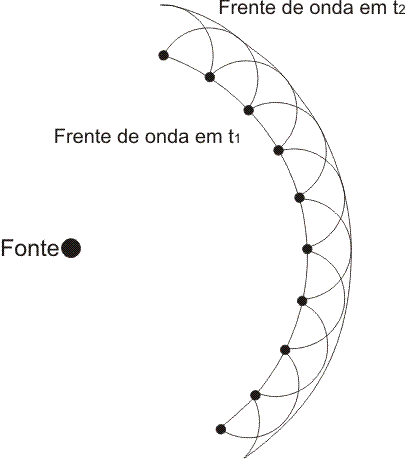
\includegraphics[width=0.4\textwidth]{huygens.png}
    \caption{Ilustração do Princípio de Huygens - a primeira linha é a frente de onda e a partir de cada ponto nessa linha é como se novas ondas fossem emitidas. A nova frente de onda será uma curva que faz a tangente em relação a essas novas ondas.}
    \label{fig:huygens}
\end{figure}

Com isso, Huygens determina que as frentes de onda se propagam como se novas ondas tivessem sido emitidas e que o conjunto dessas ondas formam a nova frente de onda e assim sucessivamente. Dessa forma, a frente de onda se propaga no espaço.

\section{Difração}
A difração é um fenômeno de quando uma onda com um comprimento de onda $\lambda$ passa por um buraco/abertura de tamanho $d$, de forma que $d\sim\lambda$.

\begin{figure}[H]
    \centering
    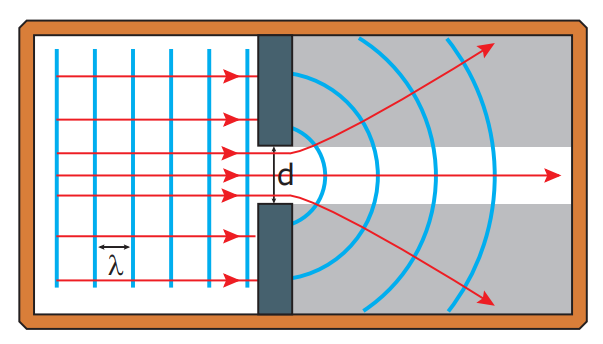
\includegraphics[width=0.6\textwidth]{difracao.png}
    \caption{Esquema da difração - quando uma onda com comprimento de onda $\lambda$ passa por um buraco ou abertura de tamanho $d$, em que $d\sim \lambda$, a onda que sai do buraco é de formato circular (caso 2D) ou esférico (caso 3D)}
    \label{fig:difracao}
\end{figure}

Um exemplo muito comum de difração é quando temos 2 pessoas conversando num corredor e você dentro de uma sala, no canto dela, consegue ouvir a conversa. Isso acontece porque a abertura do buraco da porta é de tamanho parecido com o comprimento de onda do som que emitimos ($d\sim\lambda \approx 1\,m$)  de forma que a onda sonora sofre difração ao passar pela porta.

\section{Intensidade das Ondas (I)}
Uma quantidade interessante sobre ondas é a intensidade que ondas atingem as superfícies. A intensidade das ondas (I) é definida como:
\begin{equation}
    I = \frac{P}{A}
\end{equation}
\noindent em que '$P$' é a potência da onda e '$A$' é a área da superfície (para o caso de ondas 3D) ou é o comprimento da linha que a onda atinge (para o caso de ondas 2D).

No caso de ondas circulares 2D, o comprimento da linha será o comprimento da circunferência cujo centro é o ponto de emissão da onda:
\begin{equation}
    I = \frac{P}{2\pi\,r}
\end{equation}
\noindent em que '$r$' é a distância do ponto da fonte à superfície que a onda atinge.

Para o caso de ondas esféricas, a área da superfície é a área da casca esférica em que no centro geométrico fica a fonte da onda:
\begin{equation}
    I = \frac{P}{4\pi\,r^2}
\end{equation}
\noindent em que '$r$', novamente, é a distância da fonte à superfície que a onda atinge.

Perceba que conforme a distância for maior, a intensidade das ondas 2D cai com a distância ($\sim\frac{1}{r}$), enquanto para ondas 3D, a intensidade cai com o quadrado da distância ($\sim\frac{1}{r^2}$). 

Isso acontece por causa do princípio de conservação de energia, pois a onda não pode perder nem ganhar energia. Então se eu fizer 2 superfícies de raios diferentes que englobe a fonte, a energia que passa por ambas as superfícies tem que ser iguais. Dessa forma, a intensidade que tem que diminuir para compensar.

Por isso que temos muitas antenas de telefonia móvel espalhadas pelas cidades, porque o sinal de conexão (que é a intensidade da onda que chega aos celulares) decai muito rapidamente conforme nos afastamos da antena, então precisamos de mais antenas para replicarem o sinal e aumentarem a região de cobertura do sinal.

\section{Interferência}
Interferência é o fenômenos ondulatório de interação entre 2 ou mais ondas. Uma questão importante sobre ondas é a independência das ondas, ou seja, uma onda não pode alterar/distorcer uma outra onda. Com isso, fica possível acontecer a chamada \textbf{superposição de ondas}, em que 2 ondas podem se somar momentaneamente.

\begin{figure}[H]
    \centering
    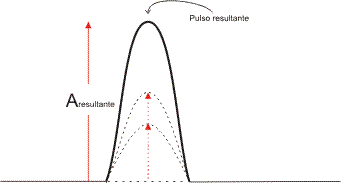
\includegraphics[width=0.6\textwidth]{superposicao.png}
    \caption{Esquema da superposição de 2 pulsos de onda. A amplitude total é a soma das amplitudes.}
    \label{fig:superposicao}
\end{figure}

Por meio da superposição, acontecem 3 tipos de interferência:
\begin{itemize}
    \item \textbf{Interferência Construtiva} - é quando 2 ondas estão superpostas e \textbf{em fase} uma com a outra, aumentando a amplitude momentaneamente. A amplitude da onda que vemos é a soma das amplitudes das ondas.
    
    \item \textbf{Interferência Destrutiva} - é quando 2 ondas estão superpostas e \textbf{em oposição de fase} uma com a outra. A amplitude da onda que vemos é a subtração das amplitudes
    
    \textbf{Interferência Mista} - é quando 2 ondas estão superpostas e defasadas entre si, mas não estão nem em fase nem em oposição de fase.
\end{itemize}

\begin{figure}[H]
    \centering
    \begin{subfigure}[b]{0.55\textwidth}
         \centering
         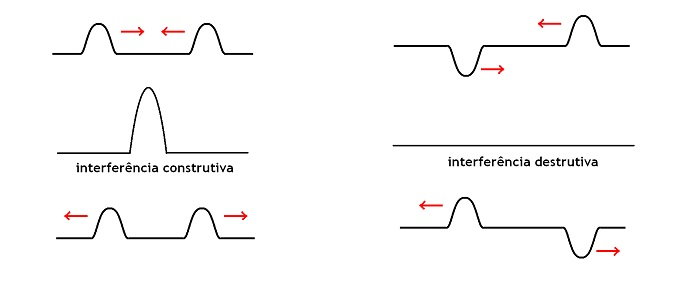
\includegraphics[height=4cm]{interferencia.jpg}
         \caption{Diagrama da interferência construtiva e destrutiva de 2 pulsos}
         \label{fig:interferencia}
     \end{subfigure}
     \hfill
     \begin{subfigure}[b]{0.4\textwidth}
         \centering
         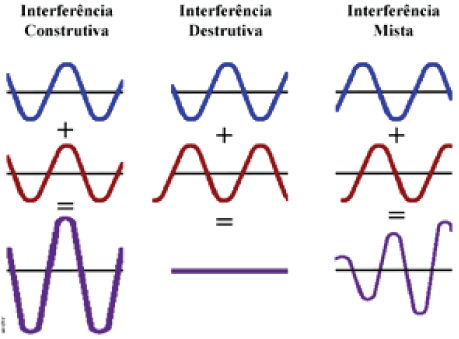
\includegraphics[width=\textwidth]{interferencia_mista.png}
         \caption{Diagrama de todas as interferências, incluindo a mista}
         \label{fig:mista}
     \end{subfigure}
    \caption{Figuras que exemplificam a interferência e como elas acontecem}
    \label{fig:interferencia_geral}
\end{figure}

\subsection{Ondas estacionárias}
Por meio da inteferência de 2 ondas, em especial 2 ondas idênticas, acontece o efeito de onda estacionária. Chamamos dessa forma, pois dá a impressão de que a onda está parada, porém é só uma ilusão ótica devido à interferência.
\begin{figure}[H]
    \centering
    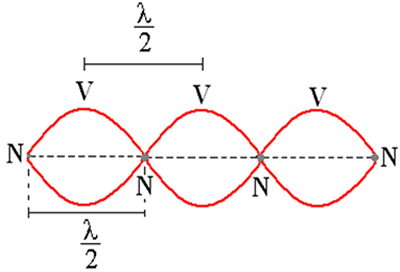
\includegraphics[width=0.6\textwidth]{estacionaria.jpg}
    \caption{Desenho de uma onda estacionária - os pontos '$N$' são chamados de \textbf{nó} e os pontos '$V$' são chamados de \textbf{ventre}.}
    \label{fig:estacionaria}
\end{figure}
Uma questão interessante das ondas é que os pontos que não se moviemntam são chamados de \textbf{nó} e a distância entre 2 nós é $\lambda/2$ (lembrar que $\lambda$ é o comprimento de onda). O ponto mais alto/baixo da onda é chamado de \textbf{ventre} e a distância entre 2 ventres também é $\lambda/2$.

As ondas estacionárias são muito úteis para o estudo de ondas em tubos, cordas e guias. Iremos utilizar essa formulação na próxima aula quando trataremos de acústica e instrumentos musicais.

\subsection{Interferência em 2D - 2 fontes coerentes}

Nessa parte, iremos entender como a interferência acontece para um caso de ondas 2D. Para isso, vamos somente nos ater ao caso em que 2 fontes são \textbf{coerentes} - ou seja as ondas emitidas por ambas fontes tem uma mesma frequência e uma diferença de fase determinada (podendo estar em fase ou em oposição de fase).

\begin{figure}[H]
    \centering
    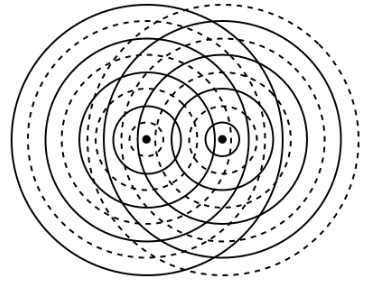
\includegraphics[width=0.6\textwidth]{interferencia_2d.png}
    \caption{Diagrama de interferência 2D - os pontos são as fontes, as linhas pontilhadas são os vales e as linhas contínuas são as cristas.}
    \label{fig:interferencia_2d}
\end{figure}
\textbf{Quando 2 vales ou 2 cristas se cruzam/interceptam, acontece a interferência construtiva. Porém, quando um vale cruza uma crista, acontece a interferência destrutiva.} Lembrando que a distância entre 2 cristas ou 2 vales é o comprimento de onda ($\lambda$).

Isso fica mais claro na figura abaixo:
\begin{figure}[H]
    \centering
    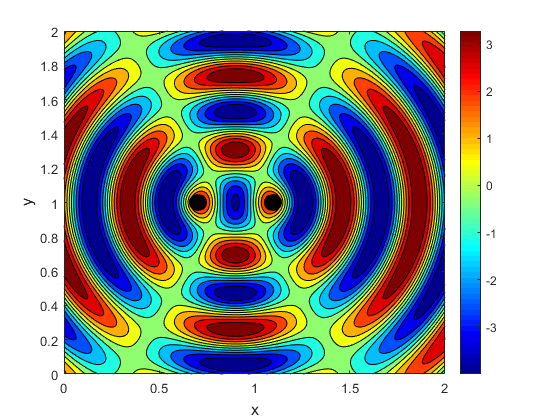
\includegraphics[width=0.8\textwidth]{interferencia_2d_color.png}
    \caption{Gráfico da interferência em 2D para 2 fontes de onda em (0.7, 1) e (1.1, 1). As bolas pretas representam os pontos em que estão as fontes.}
    \label{fig:2d_matlab}
\end{figure}
Percebam que as interferências construtivas (áreas em vermelho e azul) e as interferências destrutivas (áreas em verde) se intercalam. Além disso, existem linhas que só há interferência destrutiva. 

Esse é o princípio usado na construção de salas de teatro e de concerto musicais. Essas salas são feitas de forma que as regiões de interferência destrutivas sejam as menores possíveis para que o público possa ouvir a orquestra ou os atores e atrizes de forma perfeita.

\section{Experimento de Young (Experimento de Fenda Dupla)}
O físico Thomas Young conduziu um dos experimentos mais importantes de ótica que levou a maior compreensão de como a luz se comporta sendo onda. 

O experimento de Young é composto de uma fonte de luz, que gera frentes de onda plana, e essa frente de onda incide sobre uma parede com fenda única. Atrás da fenda, há parede com uma fenda dupla e depois há um anteparo. Abaixo está o desenho do arranjo experimental:

\begin{figure}[H]
    \centering
    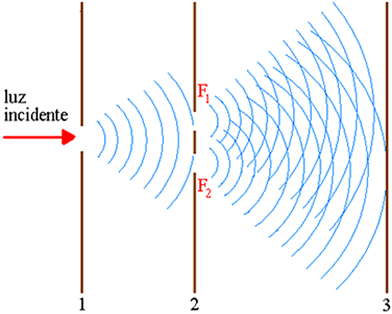
\includegraphics[width=0.6\textwidth]{fenda_dupla.jpg}
    \caption{Esquema experimental do Experimento de Young}
    \label{fig:Young}
\end{figure}
Com isso, as ondas que saem de cada fenda irá interferir com a outra da outra fenda, de forma que isso formará um padrão de interferência no anteparo (parede 3, na figura).
\begin{figure}[H]
    \centering
    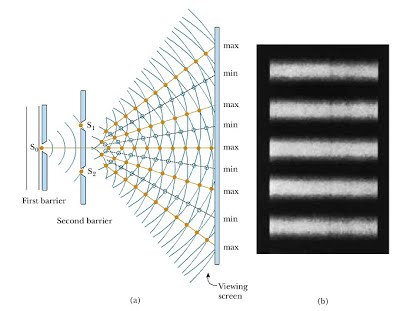
\includegraphics[width=0.8\textwidth]{young_2.jpg}
    \caption{Padrão de interferência do Experimento de Fenda Dupla. As zonas claras são as zonas de interferência construtiva e as zonas escuras são as zonas de interferência destrutiva.}
    \label{fig:young_interferencia}
\end{figure}

As frentes de interferência são dadas pela geometria:
\begin{figure}[H]
    \centering
    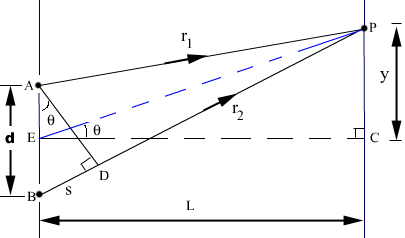
\includegraphics[width=0.6\textwidth]{young1.png}
    \caption{Desenho geométrico dos raios de luz a partir das fendas.}
    \label{fig:geometria_young}
\end{figure}
Pela geometria, $s=d\, sen \theta \approx \frac{d y}{L}$. Para que haja interferência construtiva, $s$ tem que ser uma distância múltipla do comprimento de onda, logo:
\begin{equation}
    s= n\lambda = \frac{d}{L}y \quad\quad\quad n=0,1,2,3,...
\end{equation}
\noindent em que $d$ é a distância entre as fendas, $y$ é a altura em relação ao ponto central do anteparo, $L$ é a distância entre as fendas e o anteparo e $\lambda$ é o comprimento de onda.

Para $n=0$, chamamos esse ponto como \textbf{Máximo Central}. Para $n=1$, damos ao ponto o nome de \textbf{Primeira zona de interferência} e assim por diante.

Porém, para que haja intereferência destrutiva, $s$ tem que ser uma distância múltipla do comprimento de onda da forma $\frac{1}{2}\lambda,\,\frac{3}{2}\lambda,\,\frac{5}{2}\lambda,\,\dots$. Então:
\begin{equation}
    s = \frac{n}{2}\lambda = \frac{d}{L}y \quad\quad\quad n=\frac{1}{2},\,\frac{3}{2},\,\frac{5}{2},\,\dots
\end{equation}

Dessa forma, conseguimos montar o gráfico da intensidade de luz em relação à distância ao máximo central:

\begin{figure}[H]
    \centering
    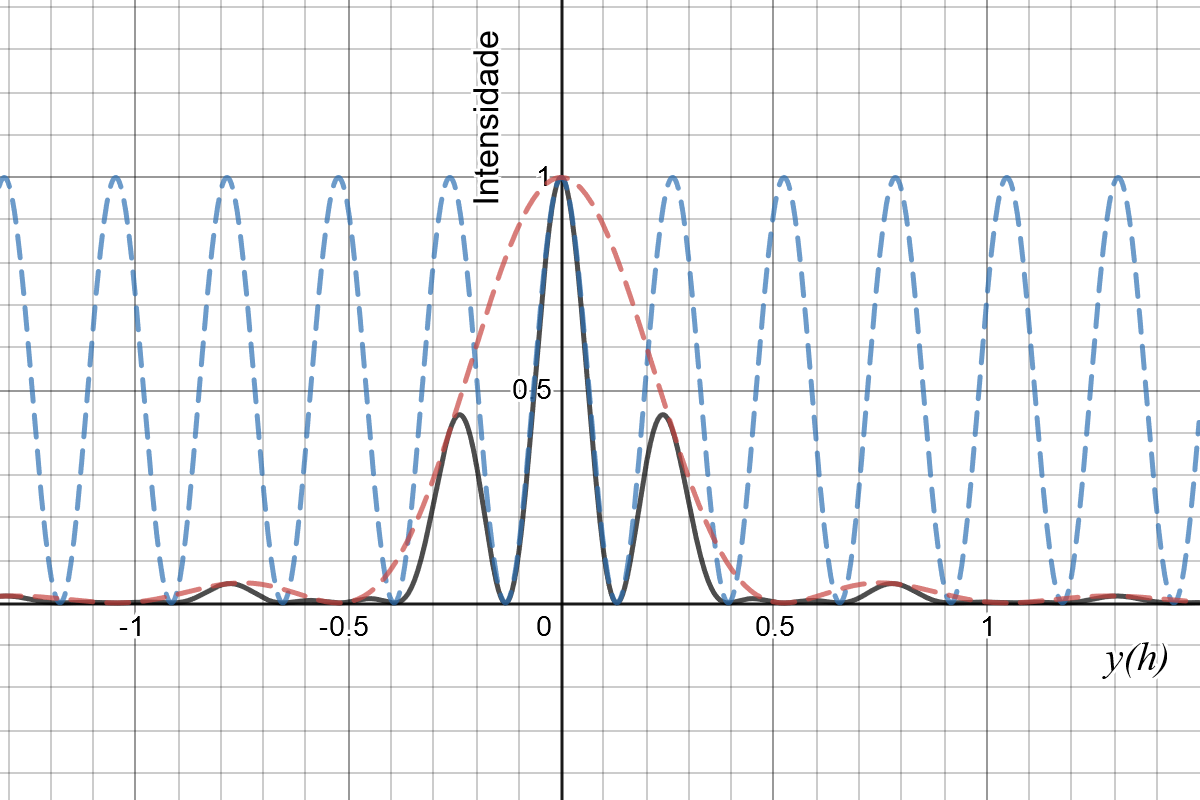
\includegraphics[width=0.9\textwidth]{padrao_inter_difracao.png}
    \caption{Gráfico da intensidade luminosa em relação do experimento de fenda dupla. Em preto está o resultado obtido, em azul está a contribuição da interferência e em vermelho está a contribuição da difração de fenda dupla.}
    \label{fig:resultado}
\end{figure}
Perceba que cada máximo do resultado bate com o máximo da interferência e os mínimos a mesma coisa, exceto para $n=3$, pois para essa caso, o resultado da difração dá 0.
\end{document}
